\section{Composing declarative static analyzers}

In this section, we propose a gneralized approach for performing declarative
static analysis for a multilingual program.

\subsection{Syntax of data-fact and rule}

First, we define the syntax of data-fact and rule, which is fairly simple.

\[e := num | string\]
\[df := p(\overline{e})\]
\[r := df :- \overline{(not)? df}\]

e stands for an element, and is either number or string.  df stands for
data-fact, and it is an ordered tuple of elements.  r stands for rule, and it
denotes how one rule can be derived from another data-facts.  It states that
LHS data-fact(the data-fact before the symbol ":-") holds if all RHS data-facts
(data-facts after the symbol ":-") without "not" notation holds, and all RHS
data-facts with "not" notation does not hold.  (? Note that recursion is
permitted, that is, a data-fact can depend on itself.  The exception is the
recursion with odd number of negation, that is, the rule such as "p(x) :- not
p(x)" is not valid. ?)

\subsection{Static analyzer for one languge}

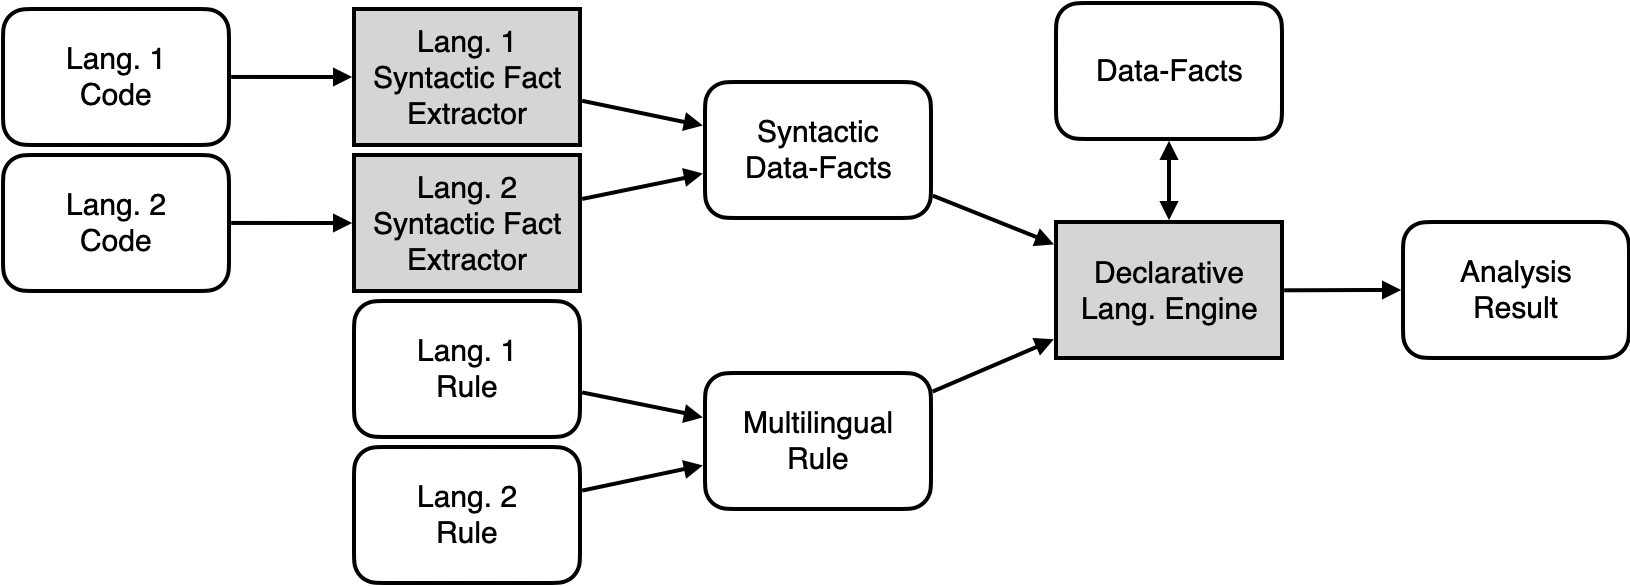
\includegraphics[width=0.5\textwidth]{img/overview}

Above figure illustrate the overview of how declarative style analysis works for
one language works. The analysis mainly
consists of three steps. First, the language is converted into a syntactic
data-facts. Second, the rules that would generate new facts are defined, and
these rules correspond to the actual implementation of the analysis. Finally, the
declarative language engine is executed with the given data-facts and rules,
giving the analysis result as an output in form of data fact.

\textbf{Extracting syntactic data-fact}
The first step is to extract syntactic data-facts from the source code.
The example of syntactic data-facts would be data-facts about certain
AST node, or parent-child relationship between nodes. For example, consider
the following code:

1 int x = 42 + 43;

We can define a data-fact of the form "expr(i, s)", which is a 2-dimensional
tuple of a number indicationg the expression id and the string representation
of that expression in the source code.  Therefore, we can extract the following
set of expr data-facts: expr(0, "42"), expr(1, "43"), and expr(2, "42 + 43"),
which indicates "42" is the 0-th expression, "43" is the 1-st, and the "42 +
43" is th 2-nd.  Another example of syntactic data-fact would be "subexpr(i, j,
k)", which is a 3-dimensional data-fact that indicates that the i-th expression
has j-th expression k-th expression. For example, we can extract the rule
subexpr(2, 0, 0) and subexpr(2, 1, 1).

In a sense, these syntactic data-facts can be viewed as building blocks for IR
of two languages.  Compared to other IRs, this declrative style of IR has a few
advantages. First, extracting in this format does not require consideration of
semantics.  It imposes almost no overhead beyond parsing the source code.
Second, the syntactic data-facts can be utilzed easily in any other kind of
analysis, since they are basically also a data-fact that can be simply
manipulated by defining new rules.  This also means that there is no need to
re-extract the syntactic data-facts, even if the different client analysis is
used.

\textbf{Defining rule}
The next step is defining rules to generate new data-facts on top of know
data-facts, that is, actually implementing the analysis in declrative style.
This setp can be futrher divided into two sub tasks. First thing to do is to
designing the generalized and unified framework for static analysis, that can
incorporate both languages. The framework consists of the result data-fact which
would correspond to the final result of the analisys, and some helper
data-facts used for calculating the result data-fact, whose implementation
would differ depending on the language. The second task is to actually fill in
the rules for such helper data-facts.

Let's look at the concrete example of dataflow analysis. First thing we do is
designing the analysis framework.  In this framework, the final analysis result
we want is expressed with the data-fact of the form of flow(a,b), which means
that value of the node a can flow into node b. flow(a, b) can be defined as
transitive closure of a data-fact step(a, b);

\[flow(a,b) :- step(a,b)\]
\[flow(a,b) :- step(a,c) and flow(c, b)\]

where the data-fact step(a,b) means that there is a direct flow from node a to b.

Next thing to do is defining rule for the helper data-fact, step, for each
language.  For example, if a lnaguage has a syntactic data-fact which indicates
the assignment x = val, in form of assign(val, x), then one can define a rule
for step to be step(a, b) :- assign(a, b).

\textbf{Defining rule}
The final step is to simply evaluate the defined rules, with the given
data-facts.  By evaluating the rules, we mean that finding all possible
data-facts that can be derived. The rules are ususally evaluated in bottom-up
and modular manner, that is, each rule is evaluated one-by-one, after every
rule it depends on is evaluated.

\subsection{Composing two static analyzers}

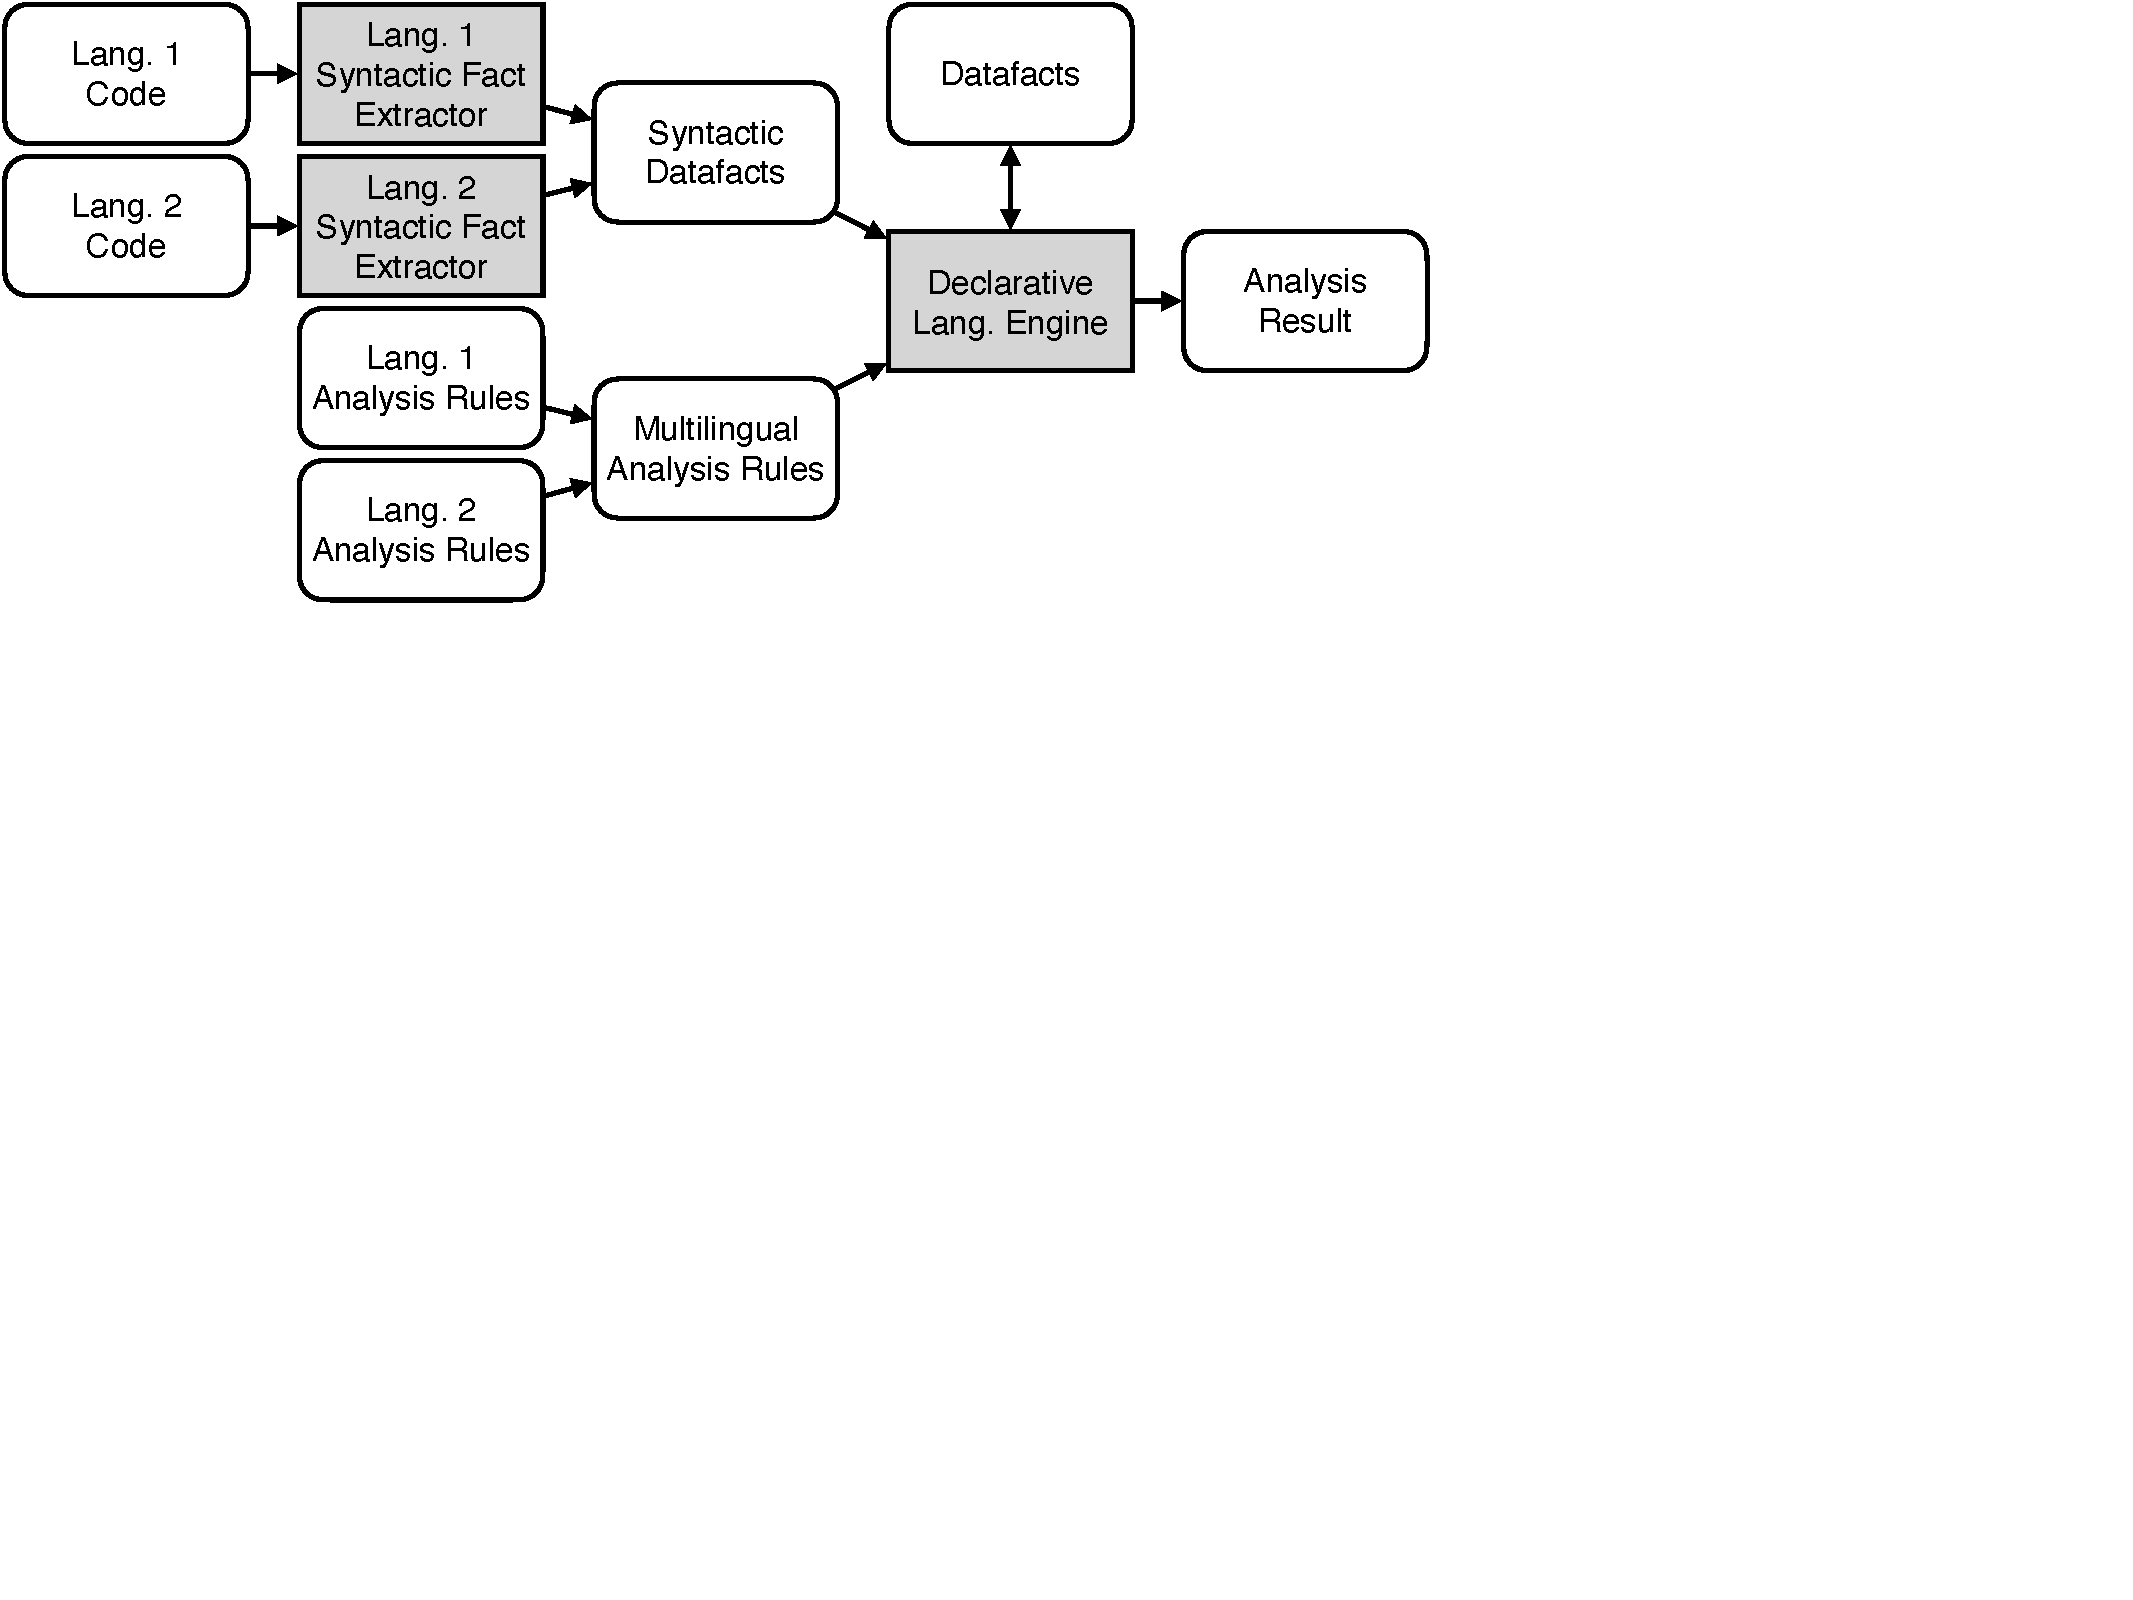
\includegraphics[width=0.5\textwidth]{img/overview2}

Above figure illustrate the overview of how declarative style analysis can
be extended to multilingual analysis. The main difference is that the evaluator
now gets two sets of syntactic data-facts extracted from both language, and
the rules also should be merged, also by taking interoperation-semantics into accout.

In order to two sets of rules, the second step can be extended with one more
task..  In the final step, the interoperation between two languages is
considered, and some helper rules in frameworks are extended to handle the
interoperation between them. By divding the second and the tird task, one can
focus on the intra-language semantics and the inter-language semantics
separately; in the second task, one can consider the task as just implementing
a static analyzer for a specific language, and in the third task, such
language-specific implementation itself needs little modification while
implementing the inter-language semantics.

Let's illustrate this step with the example of dataflow analysis above.  In
order to take the inter-language operation into account, one should find out
how a data of one language can be passed to different language beyond boudary.
A way to pass data in one language into another is via funcction call, which
can be reflected into the rule of

step(a,b) :- foreignArgParam(a,b,i)

where foreignArgParam(a,b,i) is the
data-fact that indicates a is an i-th argument of a foreign function call to a
function, whoose i-th argument is b.

There would be the trade-off between the generality of framework, and the
complexity of implementation. Designing more general framework would be easier,
yet it would require more detailed implmentaion of the framework. On the other
hand, one can design more language-specific framework which would reduce the
complexity of each helper rule, which also enables more fine-grained control
when extending helper rule to handle interoperation semantics, but designing a
good framework that is suitable for both languages would be rather challenging.

For example, we can design an alternative framework from the previous one, by
defining more fine-grained rules for step.  Assuming that both target languages
have function call and field access, step (a,b) can be defiend as

\[step(a,b) :- localStep(a, b)\]
\[step(a,b) :- functionInStep(a, b)\]
\[step(a,b) :- functionOutStep(a, b)\]
\[step(a,b) :- filedReadStep(a, b)\]
\[step(a,b) :- fieldWriteStep(a, b)\]

as a part of the framework, and define rule for each of 5 different steps.
Here, localStep represents any flows that do not envolve function call or field
access.  Example would be assigning to a variable, or simple def-use pattern.
functionInStep and functionOutStep are used for flows envolving function calls,
such as flow from argument to parameter or flows regarding return statement.
fieldReadStep and fieldWriteStep are data-facts for field access. Then, the
implementation of each framework, and the rules for inter-operation, can be
written on top of this framework. This framework has the advantage of being
modular, and rule for each framework data-facts being simpler, but designing
this framework would require the designer to verify if this design is indeed
appropriate one, i.e., both languages do have such way to pass data, and there
is no other way that a data can flow.
